\documentclass[12pt,a4paper]{article}

%\usepackage[left=1.5cm,right=1.5cm,top=1cm,bottom=2cm]{geometry}
\usepackage[in, plain]{fullpage}
\usepackage{array}
%\usepackage{../../pas-math}
\usepackage{../../moncours}



%-------------------------------------------------------------------------------
%          -Packages nécessaires pour écrire en Français et en UTF8-
%-------------------------------------------------------------------------------
\usepackage[utf8]{inputenc}
\usepackage[frenchb]{babel}
%\usepackage{numprint}
\usepackage[T1]{fontenc}
%\usepackage{lmodern}
\usepackage{textcomp}
\usepackage[french, boxed]{algorithm2e}
\usepackage{hyperref}


%-------------------------------------------------------------------------------

%-------------------------------------------------------------------------------
%                          -Outils de mise en forme-
%-------------------------------------------------------------------------------
\usepackage{hyperref}
\hypersetup{pdfstartview=XYZ}
%\usepackage{enumerate}
\usepackage{graphicx}
\usepackage{multicol}
\usepackage{tabularx}
\usepackage{multirow}
\usepackage{color}
\usepackage{eurosym}


\usepackage{anysize} %%pour pouvoir mettre les marges qu'on veut
%\marginsize{2.5cm}{2.5cm}{2.5cm}{2.5cm}

\usepackage{indentfirst} %%pour que les premier paragraphes soient aussi indentés
\usepackage{verbatim}
\usepackage{enumitem}
\usepackage{booktabs}
\usepackage[usenames,dvipsnames,svgnames,table]{xcolor}

\usepackage{variations}

%-------------------------------------------------------------------------------


%-------------------------------------------------------------------------------
%                  -Nécessaires pour écrire des mathématiques-
%-------------------------------------------------------------------------------
\usepackage{amsfonts}
\usepackage{amssymb}
\usepackage{amsmath}
\usepackage{amsthm}
\usepackage{tikz}
\usepackage{xlop}
\usepackage[output-decimal-marker={,}]{siunitx}
%-------------------------------------------------------------------------------

%-------------------------------------------------------------------------------
%                  -Nécessaires pour écrire des formules chimiquess-
%-------------------------------------------------------------------------------

\usepackage[version=4]{mhchem}

%-------------------------------------------------------------------------------
% Pour pouvoir exploiter les fichiers directement dans beamer
\newcommand{\pause}{\ }
%-------------------------------------------------------------------------------
%                    - Mise en forme avancée
%-------------------------------------------------------------------------------

\usepackage{ifthen}
\usepackage{ifmtarg}


\newcommand{\ifTrue}[2]{\ifthenelse{\equal{#1}{true}}{#2}{$\qquad \qquad$}}

%\newcommand{\kword}[1]{\textcolor{red}{\underline{#1}}}
%-------------------------------------------------------------------------------

%-------------------------------------------------------------------------------
%                     -Mise en forme d'exercices-
%-------------------------------------------------------------------------------
%\newtheoremstyle{exostyle}
%{\topsep}% espace avant
%{\topsep}% espace apres
%{}% Police utilisee par le style de thm
%{}% Indentation (vide = aucune, \parindent = indentation paragraphe)
%{\bfseries}% Police du titre de thm
%{.}% Signe de ponctuation apres le titre du thm
%{ }% Espace apres le titre du thm (\newline = linebreak)
%{\thmname{#1}\thmnumber{ #2}\thmnote{. \normalfont{\textit{#3}}}}% composants du titre du thm : \thmname = nom du thm, \thmnumber = numéro du thm, \thmnote = sous-titre du thm

%\theoremstyle{exostyle}
%\newtheorem{exercice}{Exercice}
%
%\newenvironment{questions}{
%\begin{enumerate}[\hspace{12pt}\bfseries\itshape a.]}{\end{enumerate}
%} %mettre un 1 à la place du a si on veut des numéros au lieu de lettres pour les questions 
%-------------------------------------------------------------------------------

%-------------------------------------------------------------------------------
%                    - Mise en forme de tableaux -
%-------------------------------------------------------------------------------

\renewcommand{\arraystretch}{1.7}

\setlength{\tabcolsep}{1.2cm}

%-------------------------------------------------------------------------------



%-------------------------------------------------------------------------------
%                    - Racourcis d'écriture -
%-------------------------------------------------------------------------------
%Droites
\newcommand{\dte}[1]{$(#1)$}
\newcommand{\fig}[1]{figure $#1$}
\newcommand{\sym}{symétrique}
\newcommand{\syms}{symétriques}
\newcommand{\asym}{axe de symétrie}
\newcommand{\asyms}{axes de symétrie}
\newcommand{\seg}[1]{$[#1]$}
\newcommand{\monAngle}[1]{$\widehat{#1}$}
\newcommand{\bissec}{bissectrice}
\newcommand{\mediat}{médiatrice}
\newcommand{\ddte}[1]{$[#1)$}


% Angles orientés (couples de vecteurs)
\newcommand{\aopp}[2]{(\vec{#1}, \vec{#2})} %Les deuc vecteurs sont positifs
\newcommand{\aopn}[2]{(\vec{#1}, -\vec{#2})} %Le second vecteur est négatif
\newcommand{\aonp}[2]{(-\vec{#1}, \vec{#2})} %Le premier vecteur est négatif
\newcommand{\aonn}[2]{(-\vec{#1}, -\vec{#2})} %Les deux vecteurs sont négatifs

%Ensembles mathématiques
\newcommand{\naturels}{\mathbb{N}} %Nombres naturels
\newcommand{\relatifs}{\mathbb{Z}} %Nombres relatifs
\newcommand{\rationnels}{\mathbb{Q}} %Nombres rationnels
\newcommand{\reels}{\mathbb{R}} %Nombres réels
\newcommand{\complexes}{\mathbb{C}} %Nombres complexes


%Intégration des parenthèses aux cosinus
\newcommand{\cosP}[1]{\cos\left(#1\right)}
\newcommand{\sinP}[1]{\sin\left(#1\right)}


%Probas stats
\newcommand{\stat}{statistique}
\newcommand{\stats}{statistiques}


\newcommand{\homo}{homothétie}
\newcommand{\homos}{homothéties}


\newcommand{\mycoord}[3]{(\textcolor{red}{\num{#1}} ; \textcolor{Green}{\num{#2}} ; \textcolor{blue}{\num{#3}})}
%-------------------------------------------------------------------------------

%-------------------------------------------------------------------------------
%                    - Mise en page -
%-------------------------------------------------------------------------------

\newcommand{\twoCol}[1]{\begin{multicols}{2}#1\end{multicols}}


\setenumerate[1]{font=\bfseries,label=\textit{\alph*})}
\setenumerate[2]{font=\bfseries,label=\arabic*)}


%-------------------------------------------------------------------------------
%                    - Elements cours -
%-------------------------------------------------------------------------------

%Correction d'exercice
\newcommand{\exoSec}[2]{\subsection*{Exercice #1 page #2}}
%-------------------------------------------------------------------------------
%                    - raccourcis d'écriture -
%-------------------------------------------------------------------------------

%Mise en évidence de termes clés
\newcommand{\mykw}[1]{\textcolor{red}{\underline{\textbf{#1}}}}

%Exercices
\newcommand{\exo}[2]{exercice #1 page #2}
\newcommand{\Exo}[2]{Exercice #1 page #2}

\renewcommand{\pause}{\ }




\date{}
\title{}


\begin{document}
	
\graphicspath{{./img/}}	

\chap[num=8, color=blue]{Mouvement d'un objet}{ \today }	


\begin{mypb}
	\begin{center}
		{\Large Comment caractériser le mouvement d'un objet ?}
	\end{center}
\end{mypb}


\section{Mouvement et trajectoire}

%\section{Comment caractériser un mouvement ?}

\begin{questions}
	\question Le mouvement du tunnelier est \underline{rectiligne} et \underline{uniforme}.
	
	\question Lors du fonctionnement du tunnelier, la roue coupante a une trajectoire \underline{circulaire}.
	
	\question Lors d'un cycle de fonctionnement du tunnelier la roue :
	\begin{enumerate}
		\item commence par démarrer, donc sa vitesse augmente ;
		\item puis elle se stabilise à vitesse constante;
		\item enfin elle ralenti pour s'arrêter.
	\end{enumerate} 

	\question La roue coupante du tunnelier a donc un mouvement :
	\begin{enumerate}
		\item d'abord circulaire accéléré;
		\item ensuite circulaire uniforme;
		\item enfin circulaire ralenti;
	\end{enumerate} 
\end{questions}

\begin{mybilan}
	\begin{itemize}
		\item Dans un environnement sec, un courant électrique est dangereux à partir d'une tension de 50 V.\pause
		
		\item En France, une prise électrique fournit une tension de \kw{230 V}. Il ne faut pas toucher toucher les bornes d'une prise car cela pourrait provoquer une \kw{électrisation} voire une \kw{électrocution}.\pause
				 
	\end{itemize}

\end{mybilan}

\begin{mydefs}
	\begin{itemize}
		\item \kw{\'Electrisation} : passage du courant électrique à travers le corps humain. 
		
		\item \kw{\'Electrocution} : \'electrisation qui entraine la mort.
	\end{itemize}
\end{mydefs}




\begin{myexos}
	\begin{itemize}
		
		\item \exo{6}{55}  : relativité du mouvement.
		\item \exo{8}{56}  : définition trajectoire.
		\item \exo{9}{56}  : Choix d'un référentiel (en anglais).
		\item \exo{10}{56} : relativité du mouvement, choix du référentiel.
		\item \exo{11}{56} : un même mouvement, deux points de vue (référentiel)
		\item \exo{13}{56} : QCM référentiels et trajectoire
	\end{itemize}
\end{myexos}

\section{Vitesse d'un objet}

%\begin{myact}{}

		Activité 16 page 51 cahier d'activités

\end{myact}

\begin{mybilan}
	\begin{itemize}
		\item L'énergie peut être \kw{transférée} d'un objet vers un autre objet.
		
		\item Une forme d'énergie peut être \kw{convertie} en une autre forme d'énergie.
		
		
		\begin{center}
			\includegraphics[scale=0.8]{conversion}
		\end{center}
		
		\item On représente un ensemble de transferts et conversions d'énergie par une \kw{chaine énergétique}.

		\begin{center}
			\includegraphics[scale=0.5]{chaine}
		\end{center}
	\end{itemize}
\end{mybilan}






\begin{myexos}
	\begin{itemize}
		\item \exo{5}{55}  : vitesses et unités
		\item \exo{7}{55}  : mots croisés bilan
		\item \exo{12}{56} : référentiel, trajectoire et vitesse
		\item \exo{14}{56}  : Calculs de vitesse et graphique		
		\item \exo{12}{56}  : Calculs de vitesse, conversions, type mouvement	
	\end{itemize}
\end{myexos}

\begin{center}
	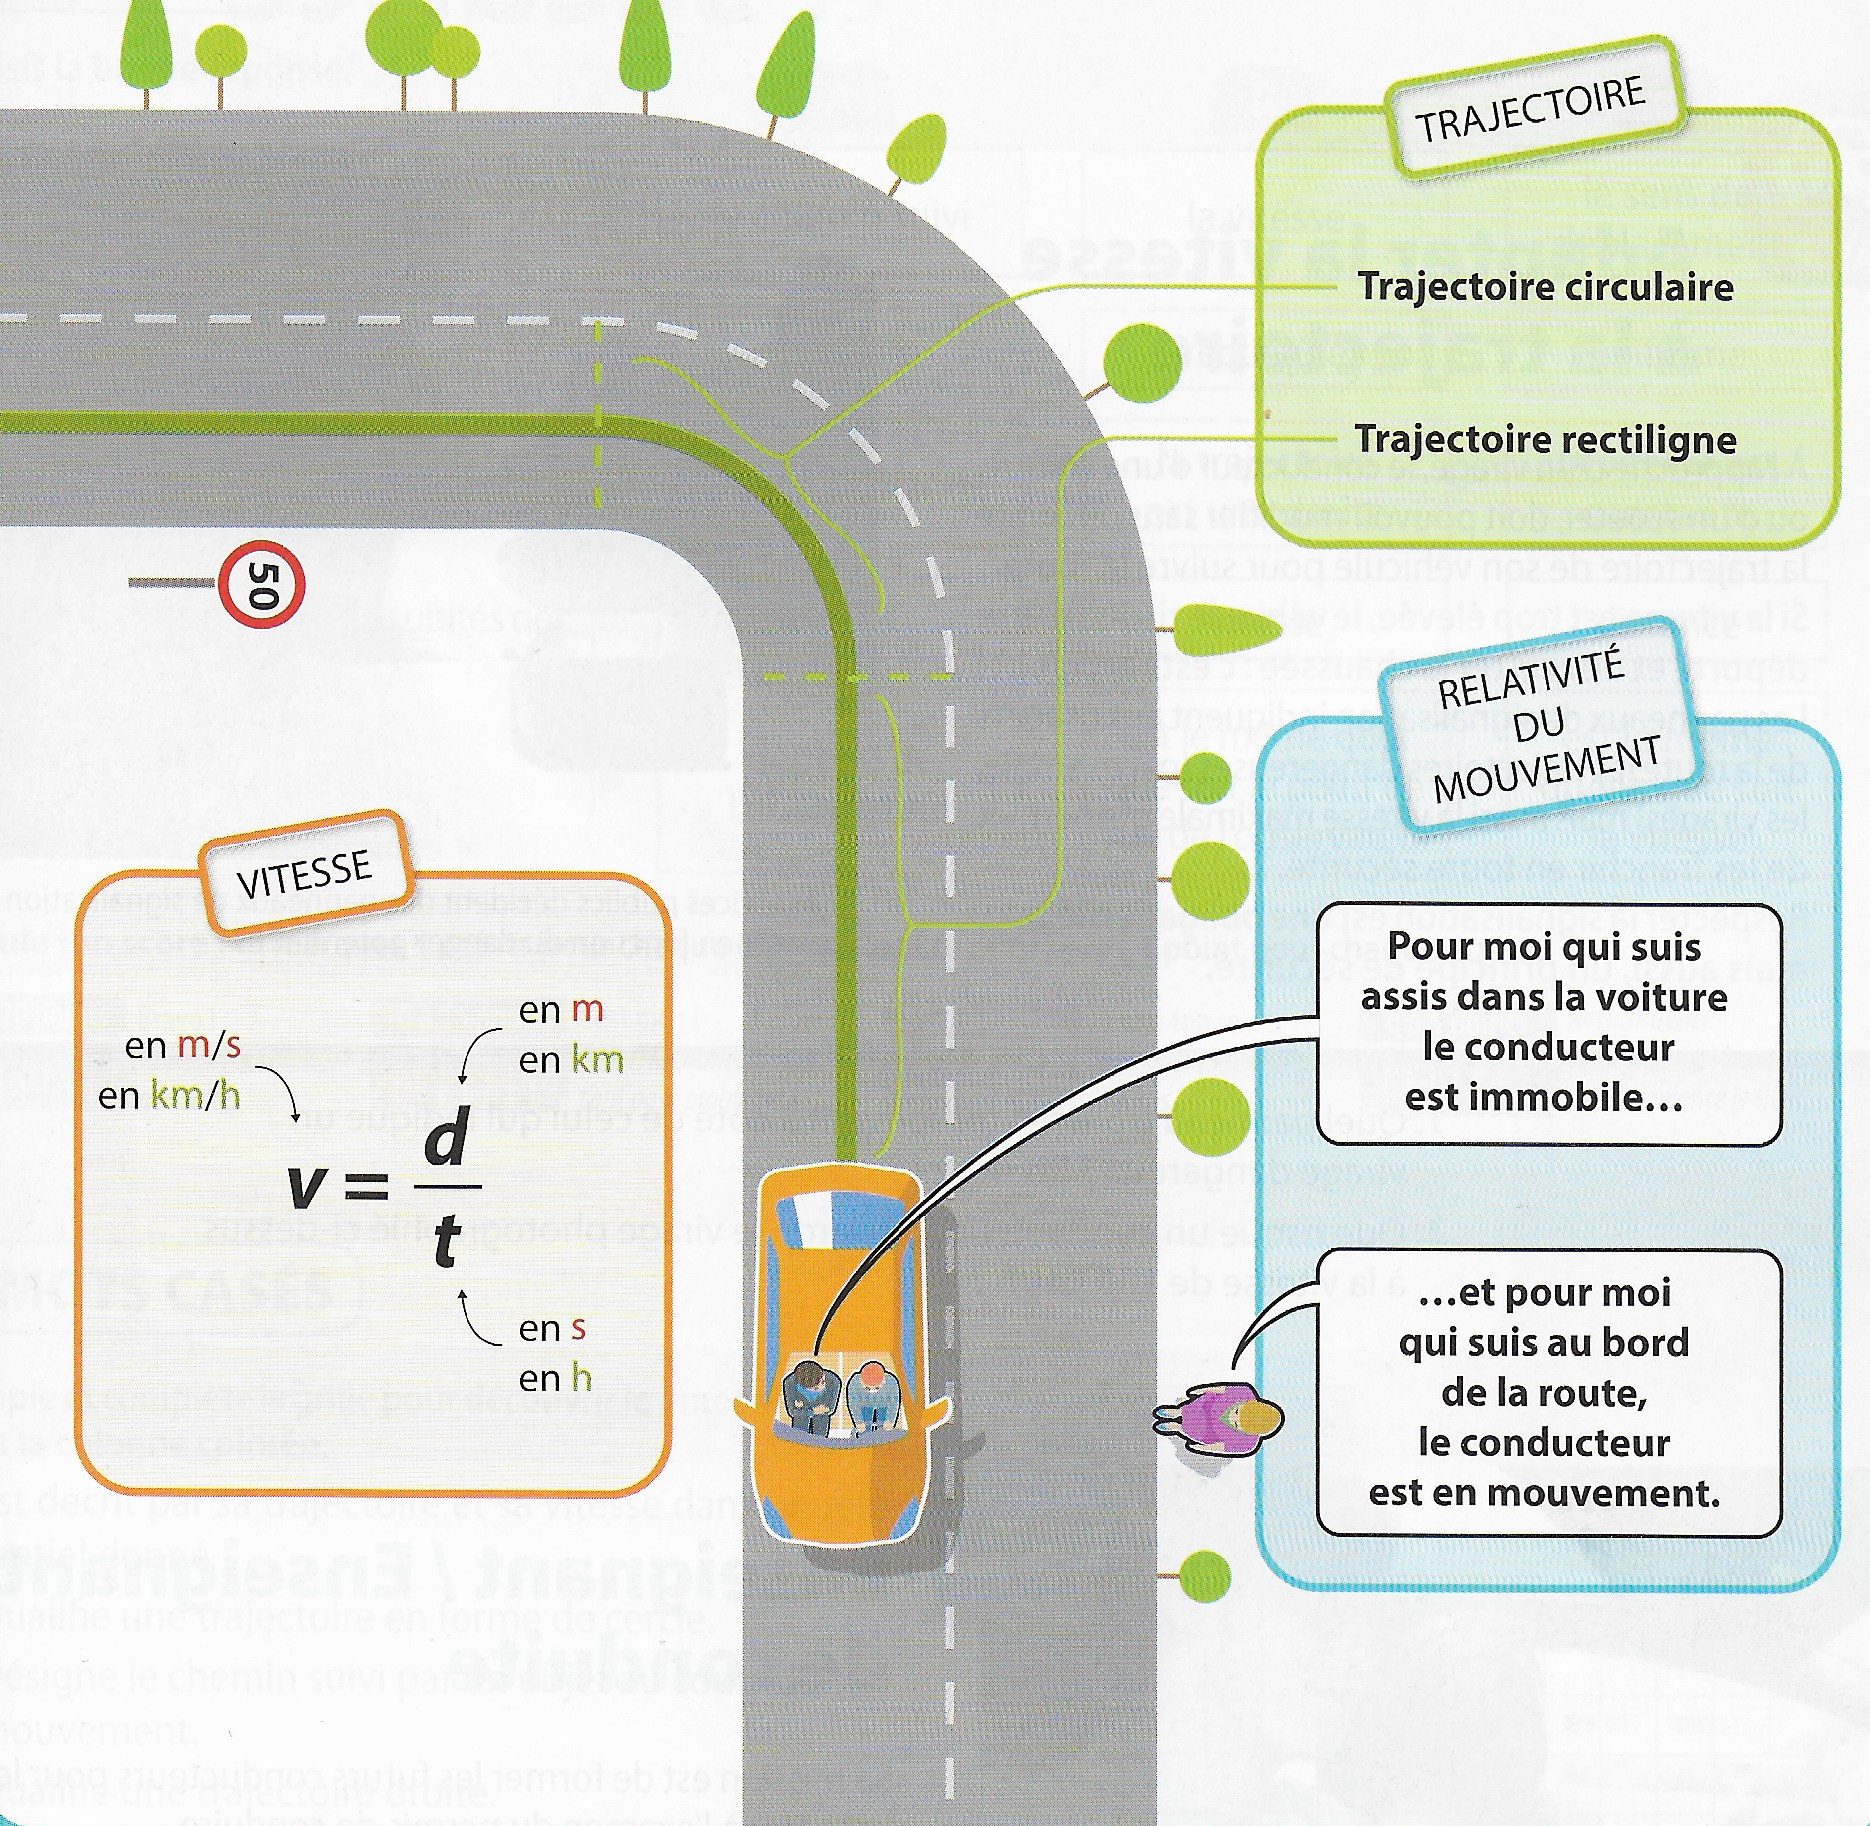
\includegraphics[scale=0.7]{img/bilan}
\end{center}

\appendix

%\newpage


\end{document}